\documentclass[]{report}
\usepackage{kotex}
\usepackage{verbatim} 
\usepackage{graphicx} 

\usepackage{listings}
\usepackage{color}

\definecolor{dkgreen}{rgb}{0,0.6,0}
\definecolor{gray}{rgb}{0.5,0.5,0.5}
\definecolor{mauve}{rgb}{0.58,0,0.82}

\lstset{frame=tb,
	language=Python,
	aboveskip=3mm,
	belowskip=3mm,
	showstringspaces=false,
	columns=flexible,
	basicstyle={\small\ttfamily},
	numbers=none,
	numberstyle=\tiny\color{gray},
	keywordstyle=\color{blue},
	commentstyle=\color{dkgreen},
	stringstyle=\color{mauve},
	breaklines=true,
	breakatwhitespace=true,
	tabsize=3
}


% Title Page
\title{HW05 - REPORT}
\author{정보컴퓨터공학부 201624536 이국현}


\begin{document}
\maketitle


\chapter{서론}
\begin{itemize}
	\item Projection
	\item Homography
	\item RANSAC
\end{itemize} 

\section{Projection}

\begin{figure}[ht!]
	\centering
	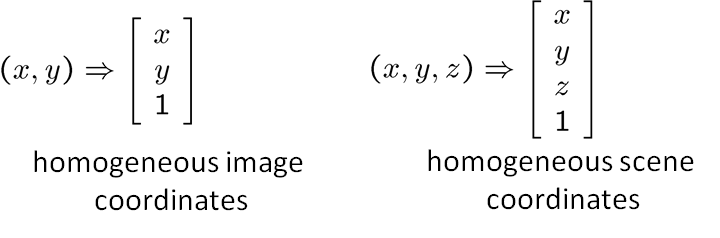
\includegraphics[width=0.9\textwidth]{image/image_to_homogeneous.png}
	\caption{Image to homogeneous}
	\label{image_to_homogeneous}
\end{figure}

Source image를 reference image의 coordinate로 변환하기 위해 Homography matrix를 곱하려면 
먼저 Source image를 homogeneous coordinate로 변환해야 한다. 
이는 그림과 같이 Additional dimension을 주어 변환할 수 있다. \\

\begin{figure}[ht!]
    \centering
    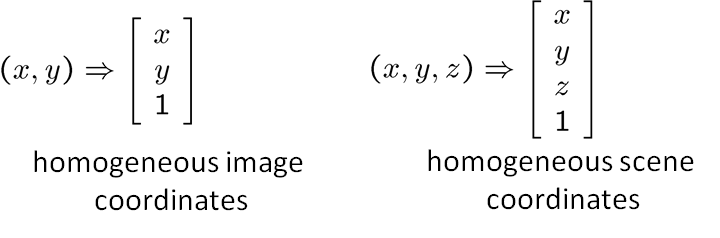
\includegraphics[width=0.9\textwidth]{image/image_to_homogeneous.png}
    \caption{Image to homogeneous}
    \label{image_to_homogeneous}
\end{figure}

Homography matrix 연산을 수행하였다면, 다시 Homogeneous coordinate를 Image coordinate로 변환해야 한다. 
이는 그림과 같이 Additional dimension을 제거하고, 그 값으로 Nomalize 하면 된다. \\

\section{Homography}

\begin{figure}[ht!]
	\centering
	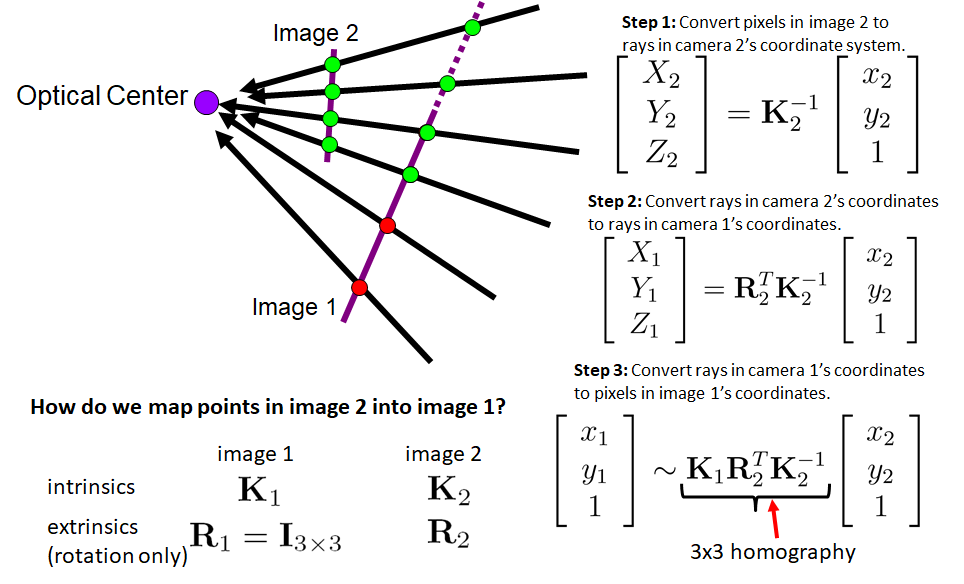
\includegraphics[width=1\textwidth]{image/homography_matrix.png}
	\caption{Homography matrix}
	\label{homography_matrix}
\end{figure}

Homography matrix는 Intrinsics과 Transformation을 표현하는 Extrinsics으로 구성되어 있으며, 
한 Image coordinate에서 다른 Image coordinate로 변환하는 과정을 포함하고 있다. \\

\section{RANSAC}

Panorama를 생성하기 위해서는 Image 간의 Homography matrix를 계산해야 하며,
이를 위해 Image 간의 Feature를 매치하지만, Outlier가 생길 수 있다. 
이 Outlier는 Panorma를 생성하는 데 큰 장애물이 될 수 있기 때문에 RANSAC을 이용하여 Outlier를 제거한다. 
RANSAC의 알고리즘은 다음과 같다. \\

\begin{enumerate}
	\item Feature Matches에서 랜덤으로 필요한 만큼의 Match set을 선택하여 Model 생성 \\
        이때 필요한 Match의 수는 Transformation의 특성에 따라 다르다. 
	\item 각 Model에서 Transformation 구한다 (Homography matrix)
	\item 각 Model에서의 Inlier counting
	\item 1 - 3을 반복
	\item Inlier가 가장 많은 Model 선택
	\item 새로운 Model에서 Outlier 제거
	\item 추출된 Inlier로 다시 최종 Model 생성 \\
\end{enumerate}

\chapter{본론}

\section{Keypoint Projection}

\begin{lstlisting}
    def KeypointProjection(xy_points, h):
    assert isinstance(xy_points, np.ndarray)
    assert isinstance(h, np.ndarray)
    assert xy_points.shape[1] == 2
    assert h.shape == (3, 3)
    
    # START
    h_points = []
    for xy_point in xy_points:
    # image coordinate를 homogeneous coordinate로 변환
    h_point = np.append(xy_point, 1)
    h_points.append(h_point)
    h_points = np.array(h_points)
    
    xy_points_out = []
    for h_point in h_points:
    # homography matrix를 곱하여 reference coordinate로 변환
    xy_point_out = h.dot(h_point)
        nomalizer = xy_point_out[2] if (xy_point_out[2] != 0) else 1e-10
        # additional dimension을 없애고 그 값으로 나누어 projection
        xy_point_out = xy_point_out[:2] / nomalizer
        xy_points_out.append(xy_point_out)
        xy_points_out = np.array(xy_points_out)
        # END
        return xy_points_out
    \end{lstlisting}

Source image를 Reference image의 coordinate로 변환하기 위해 먼저, Source image를 Homogeneous coordinate로 변환하고,
여기에 Homography matrix를 곱하여 Reference image의 Coordinate로 변환하였다. 마지막으로 Additional dimension을 없애면서 해당 값으로 나누어 Nomalize 해주었다.\\


\section{RANSAC}

Panorama를 생성하기 위해서 Image 간의 Feature를 매치하지만,
Outlier가 생길 수 있고, 이 Outlier가 Panorma를 생성하는 데 큰 장애물이 될 수 있기 때문에,
RANSAC을 이용하여 Outlier를 제거한다. \\ 

\begin{lstlisting}
def RANSACHomography(xy_src, xy_ref, num_iter, tol):
    assert isinstance(xy_src, np.ndarray)
    assert isinstance(xy_ref, np.ndarray)
    assert xy_src.shape == xy_ref.shape
    assert xy_src.shape[1] == 2
    assert isinstance(num_iter, int)
    assert isinstance(tol, (int, float))
    tol = tol * 1.0

    # START
    minMatchCount = 4  # homography matrix를 구하기 위해 최소 4개의 match가 필요
    maxCount = 0
    maxMatches = 0
    for k in range(num_iter):
        matches = []
        # random으로 4개의 match 선택
        for _ in range(minMatchCount):
            match = random.randint(0, len(xy_src) - 1)
            matches.append(match)
        # 선택한 match로 homography matrix를 구하고 proejction
        h, _ = cv2.findHomography(xy_src[matches], xy_ref[matches])
        xy_proj = KeypointProjection(xy_src, h)

        inlierCount = 0
        # 모든 match를 순회하여 inlier counting
        for i in range(xy_proj.shape[0]):
            dist = np.linalg.norm(xy_proj[i] - xy_ref[i])
            if dist < tol:
                inlierCount += 1
        # inlier가 가장 많은 match set 선택
        if inlierCount > maxCount:
            maxCount = inlierCount
            maxMatches = matches

    # inlier가 가장 많은 match set으로 homography matrix를 구하고 proejction
    h, _ = cv2.findHomography(xy_src[maxMatches], xy_ref[maxMatches])
    xy_proj = KeypointProjection(xy_src, h)
    # inlier 추출
    inliers = []
    for i in range(xy_proj.shape[0]):
        dist = np.linalg.norm(xy_proj[i] - xy_ref[i])
        if dist < tol:
            inliers.append(i)
    # inlier를 가지고 다시 homography matrix를 구해서 return
    h, _ = cv2.findHomography(xy_src[inliers], xy_ref[inliers])
    # END
    assert isinstance(h, np.ndarray)
    assert h.shape == (3, 3)
    return h
\end{lstlisting}

수행한 RANSAC의 단계는 다음과 같다. \\

\begin{enumerate}
	\item Matches에서 랜덤으로 4개 이상의 Match 선택
	\item 선택한 Match set으로 Homography matrix 생성
	\item Eucleadian distance를 통해 Inlier counting (tol보다 작을 때)
	\item 1 - 3을 num\_iter 번 반복
	\item Inlier가 가장 많은 Homography matrix 선택
	\item 새로운 Homography matrix에서 Outlier 제거
	\item 추출된 Inlier로 다시 최종 Homography matrix 생성 \\
\end{enumerate}

\chapter{결론}

\section{Keypoint Projection}

\begin{figure}[ht!]
	\centering
	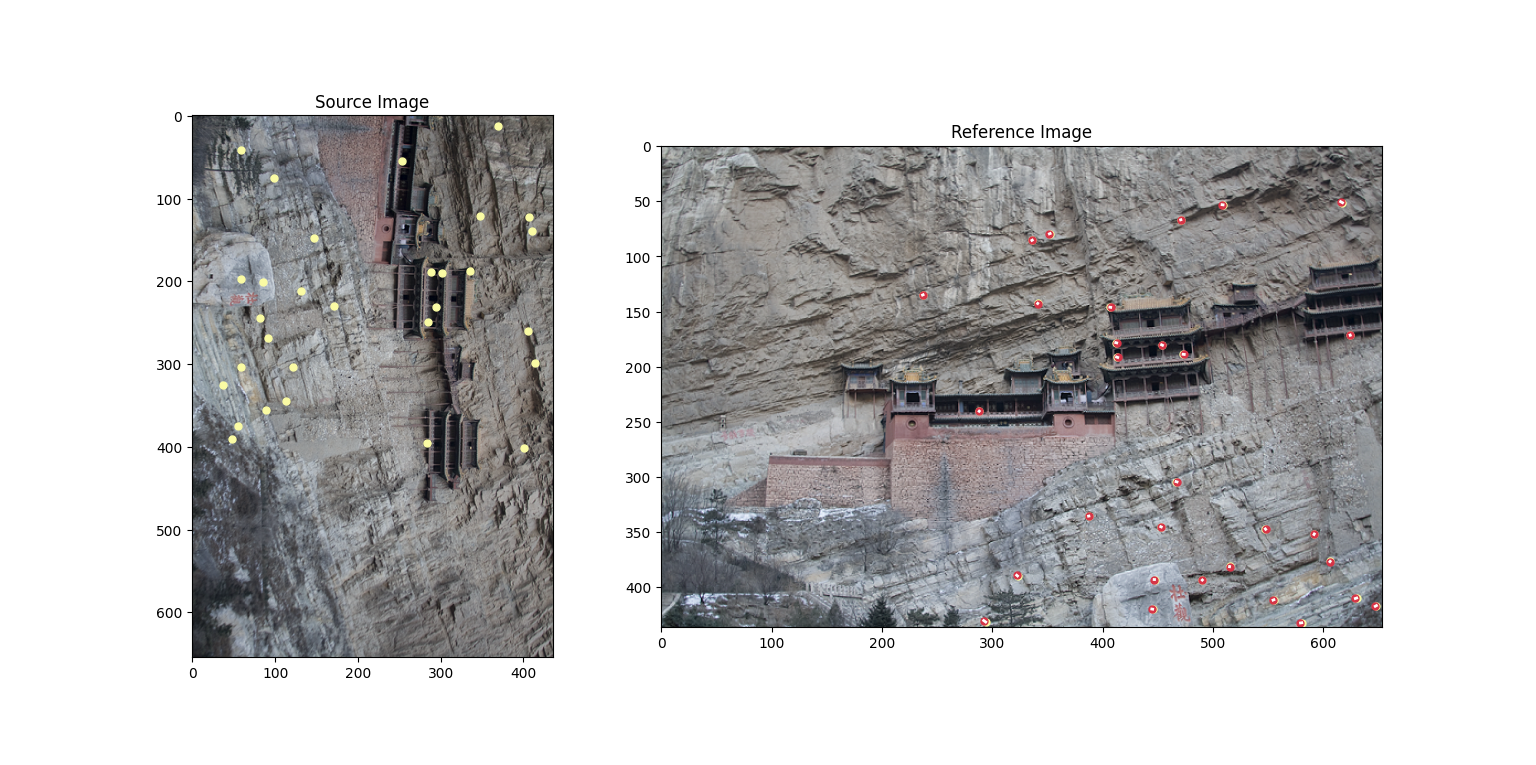
\includegraphics[width=1\textwidth]{image/Hanging1-Hanging2.png}
	\caption{Keypoint Projection}
	\label{Hanging1-Hanging2}
\end{figure}

Source Image의 Feature들이 Reference frame으로 Projection 되어 매칭된 것을 확인할 수 있다. \\


\section{RANSAC}

\begin{figure}[ht!]
	\centering
	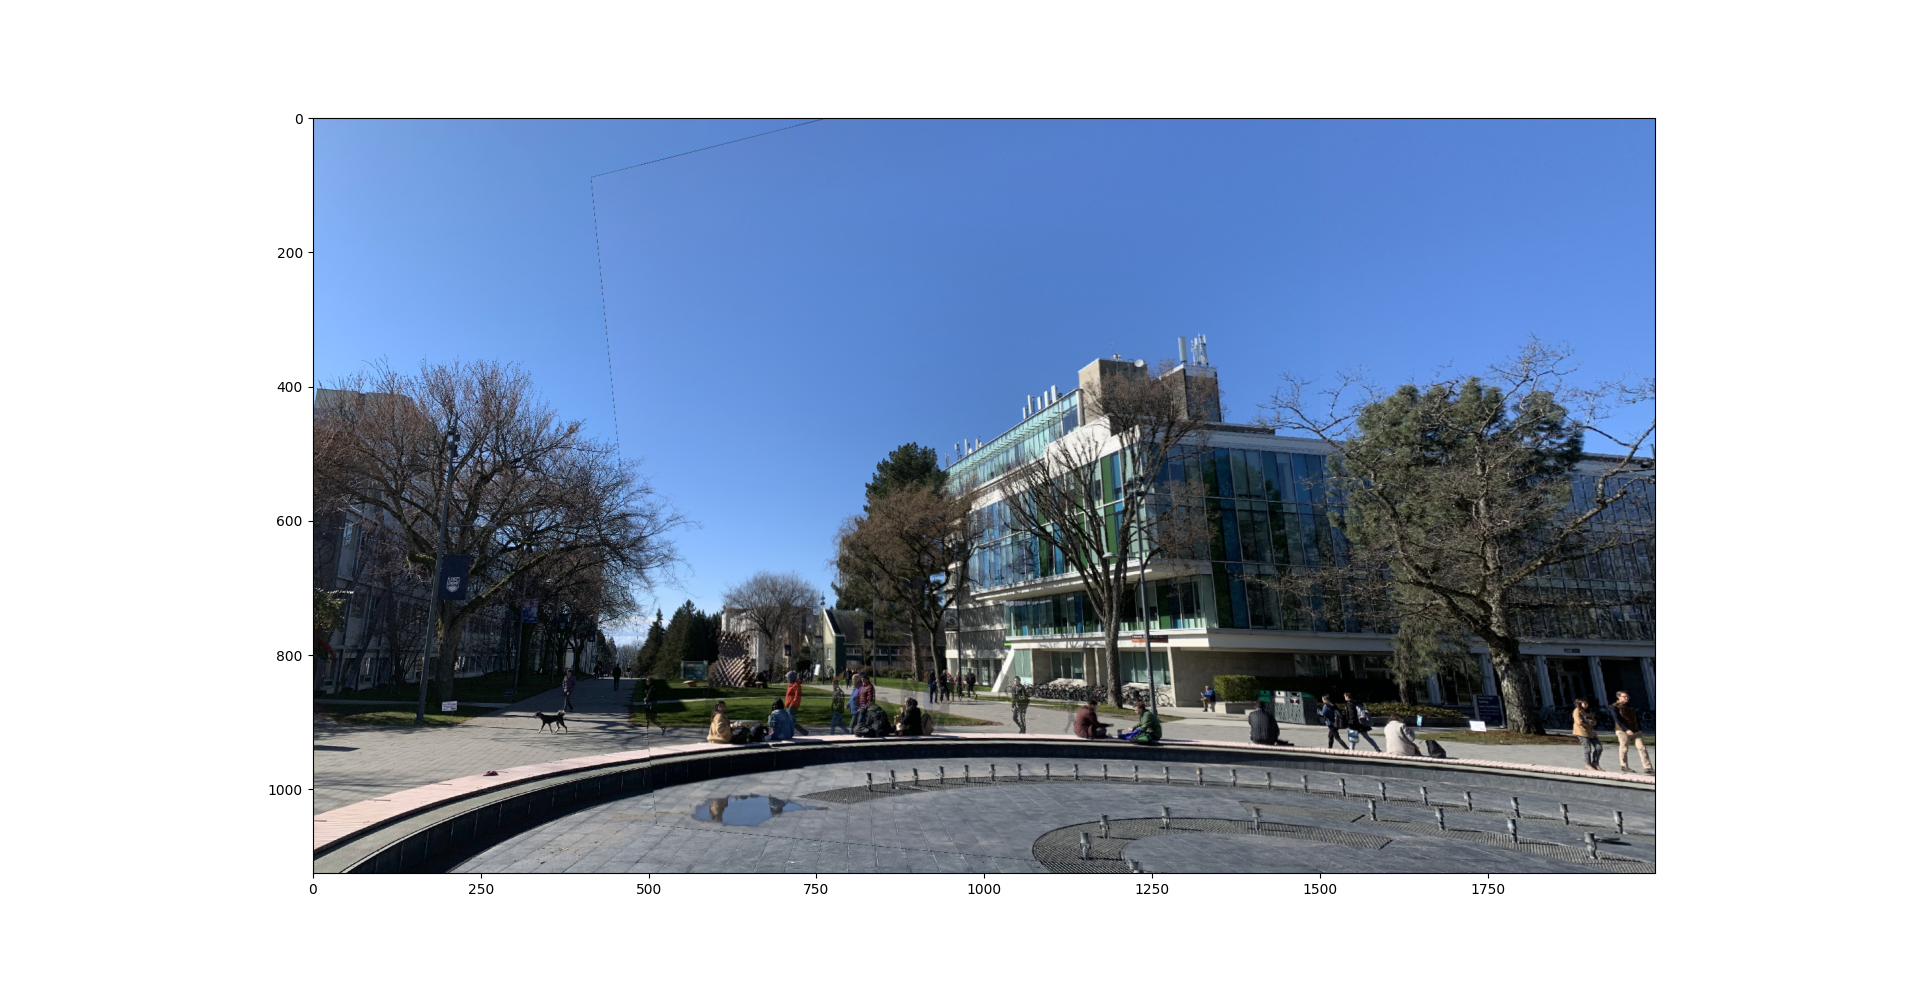
\includegraphics[width=1\textwidth]{image/fountain4-fountain0.png}
	\caption{fountain}
	\label{fountain4-fountain0}
\end{figure}

Fountain의 경우 num\_iter=70, tol=20으로 설정하였을 때 좋은 Panorama image를 얻을 수 있었다. \\

\begin{figure}[ht!]
	\centering
	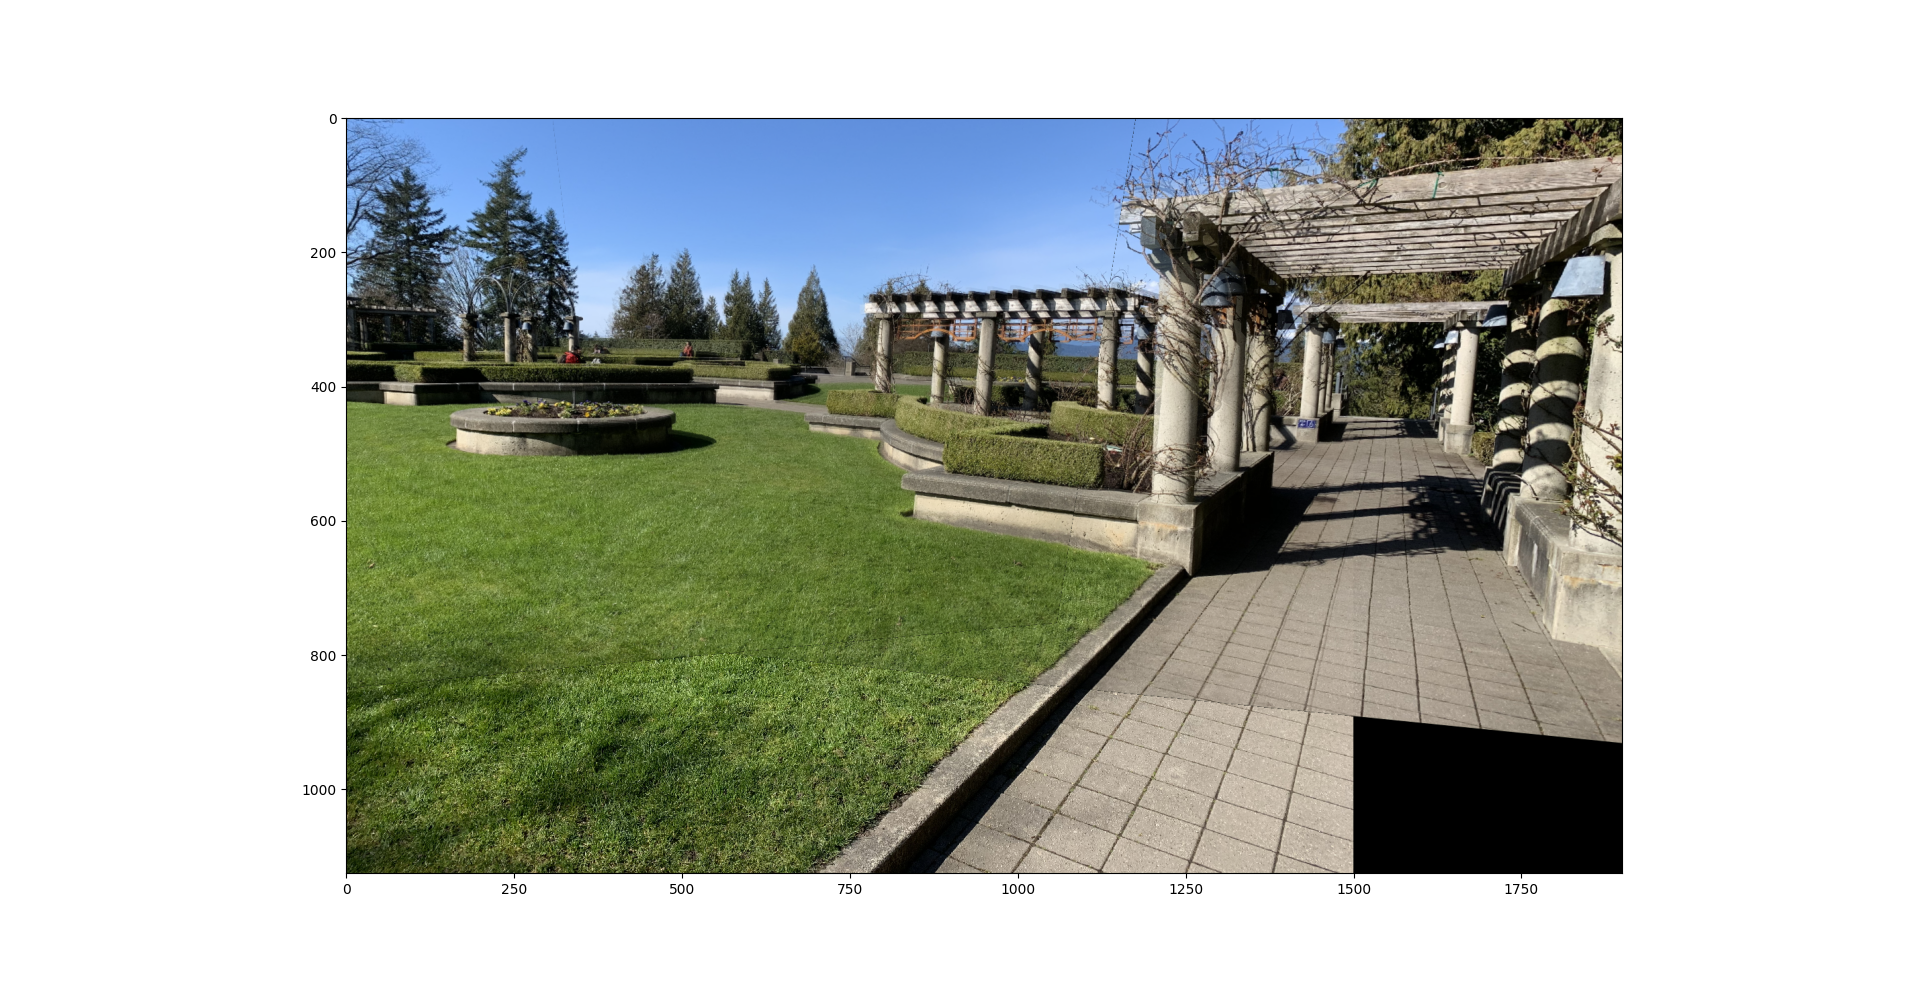
\includegraphics[width=1\textwidth]{image/garden0-garden3-garden4.png}
	\caption{garden}
	\label{garden0-garden3-garden4}
\end{figure}

Garden의 경우 num\_iter=400, tol=15으로 설정하였을 때 좋은 Panorama image를 얻을 수 있었다. \\

\begin{figure}[ht!]
	\centering
	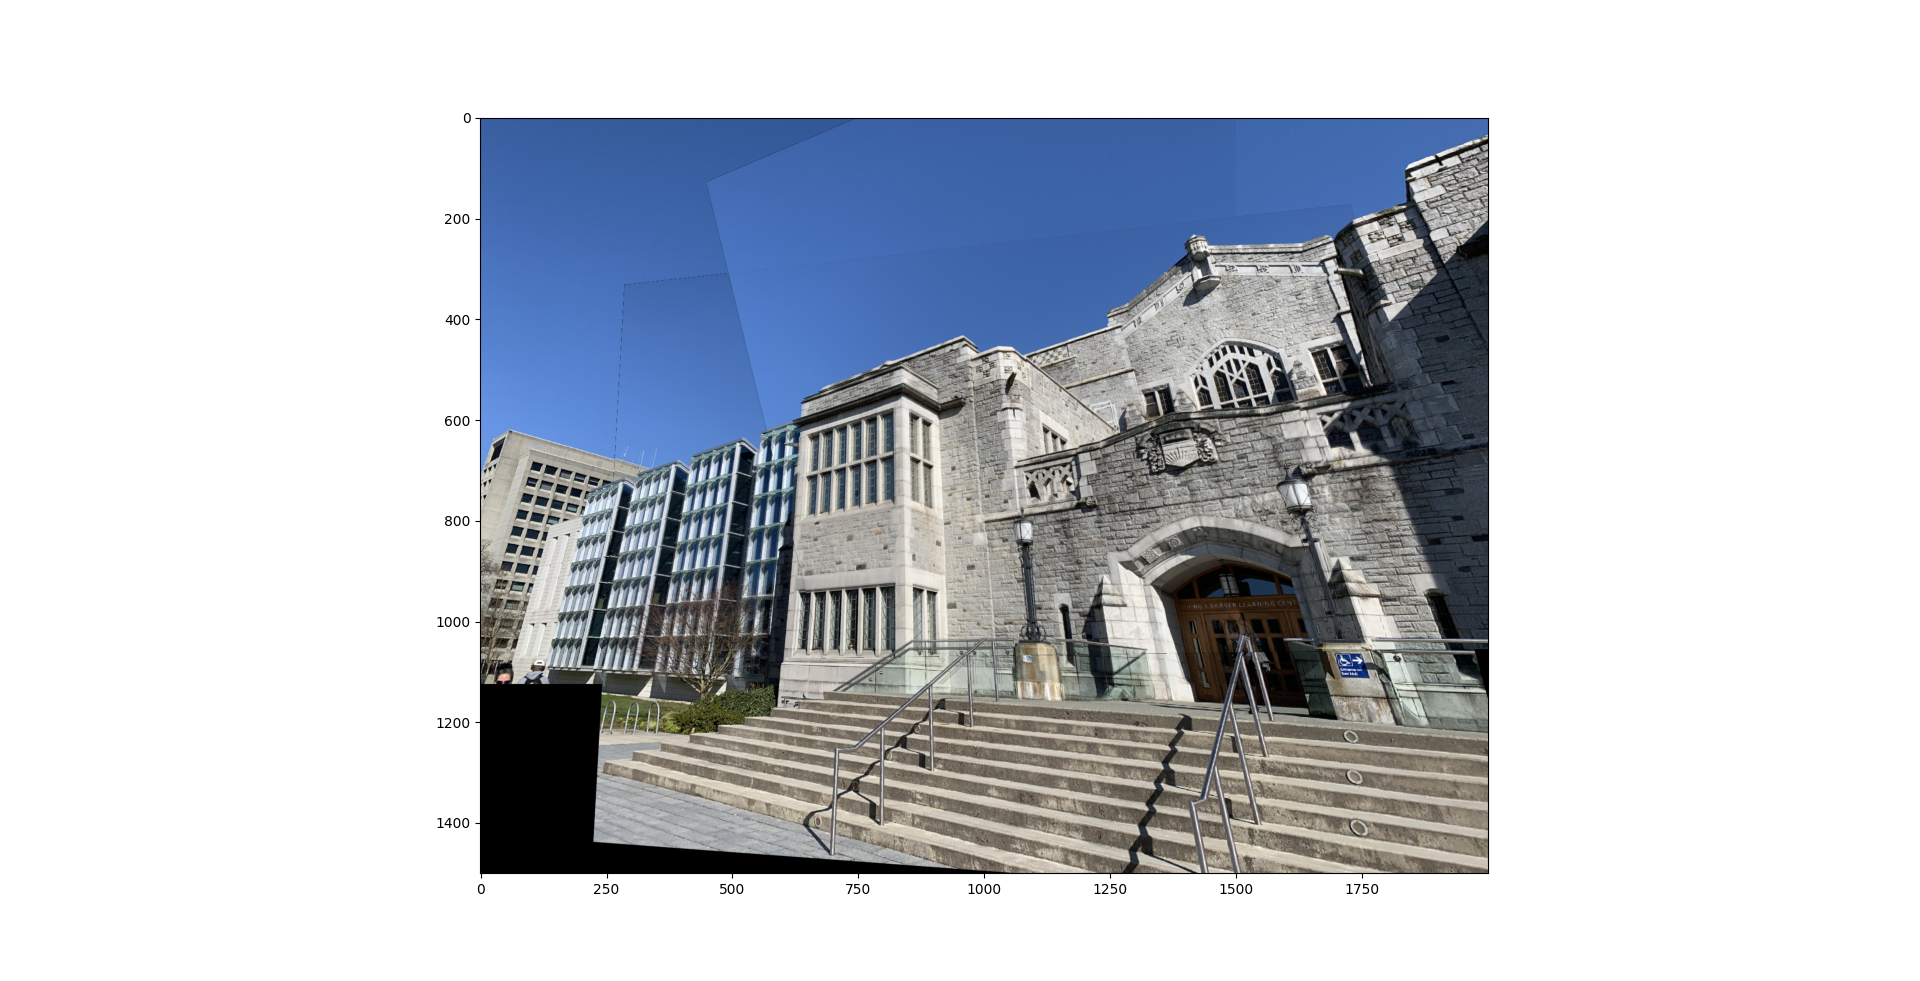
\includegraphics[width=1\textwidth]{image/irving_out3-irving_out6-irving_out5.png}
	\caption{irving}
	\label{irving_out3-irving_out6-irving_out5}
\end{figure}

Iriving의 경우 Outlier Ratio는 num\_iter=70, tol=20으로 설정하였을 때 좋은 Panorama image를 얻을 수 있었다. \\


\section{Parameter setting}

\[ N >= \frac{\log{(1-p)}}{\log{(1 - (1 - e)^s )}} \]

\begin{itemize}
	\item p : Target Accuracy
	\item e : Proportion of outliers
	\item s : Least sample size
\end{itemize} 

Interation number N은 위와 같은 수식으로 결정할 수 있다. 
Outlier ratio는 설정한 Interation number와 Tolerance에 따라 달라질 수 있기 때문에, 
자동화를 통해 따라 여러 값을 테스트해 봐야 할 것이다. 
Accuracy rate를 0.7 이상으로 설정하여 구한 Interation number를 사용하였을 때, 시각적으로 잘 연결된 Panorama image를 얻을 수 있었다. \\

\end{document}      